\documentclass[12pt]{article}
\usepackage{geometry}
\geometry{verbose,a4paper,tmargin=1in,bmargin=1in,lmargin=1in,rmargin=1in}
\usepackage{graphicx}

\title{Getting started with the AHIR tools}
\author{Sameer D. Sahasrabuddhe}
\date{February 2008}

\begin{document}

\maketitle

\section{Overview}

The compilation flow that generates an AHIR circuit specification from
an input C program is a three-stage process:
\begin{enumerate}
  \item parsing the C program using a standard compiler front-end
        (\texttt{llvm-gcc}, provided by LLVM)
  \item generating an unlinked AHIR specification from the compiler's
        standard IR (\texttt{irgen}, implemented using LLVM)
  \item linking the AHIR specification and generating a memory map that
        is assumed by the linked circuit (\texttt{irlink})
\end{enumerate}

\begin{figure}[htb]
  \centering
  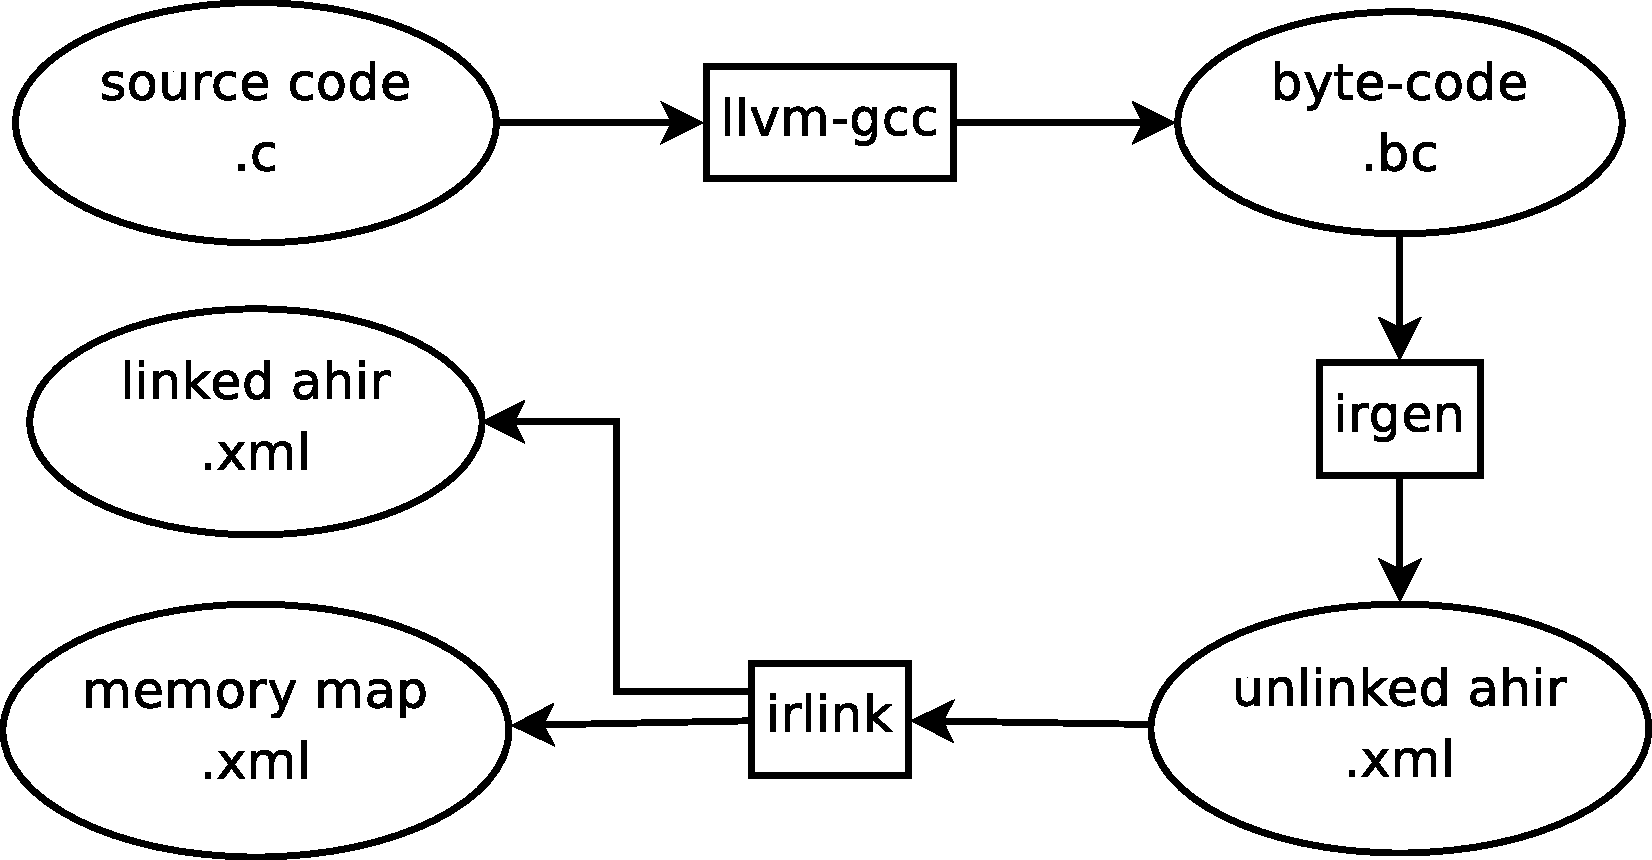
\includegraphics[keepaspectratio,width=4in]{images/source-to-ahir.pdf}
  \caption{Compiling input source to AHIR}
  \label{figure:source-to-ahir}
\end{figure}

The linker stage is meant to allow separate compilation of ``source
libraries''. For now the tools only process a single standalone C
file, that must include all the functions required to create a complete
working application.

%The tools that process the linked AHIR specification are all
%standalone AHIR tools, that do not depend on any other project
%framework. Primary operations to be performed on the specification are
%analysis, optimisation, simulation and synthesis.

\begin{figure}[htb]
  \centering
  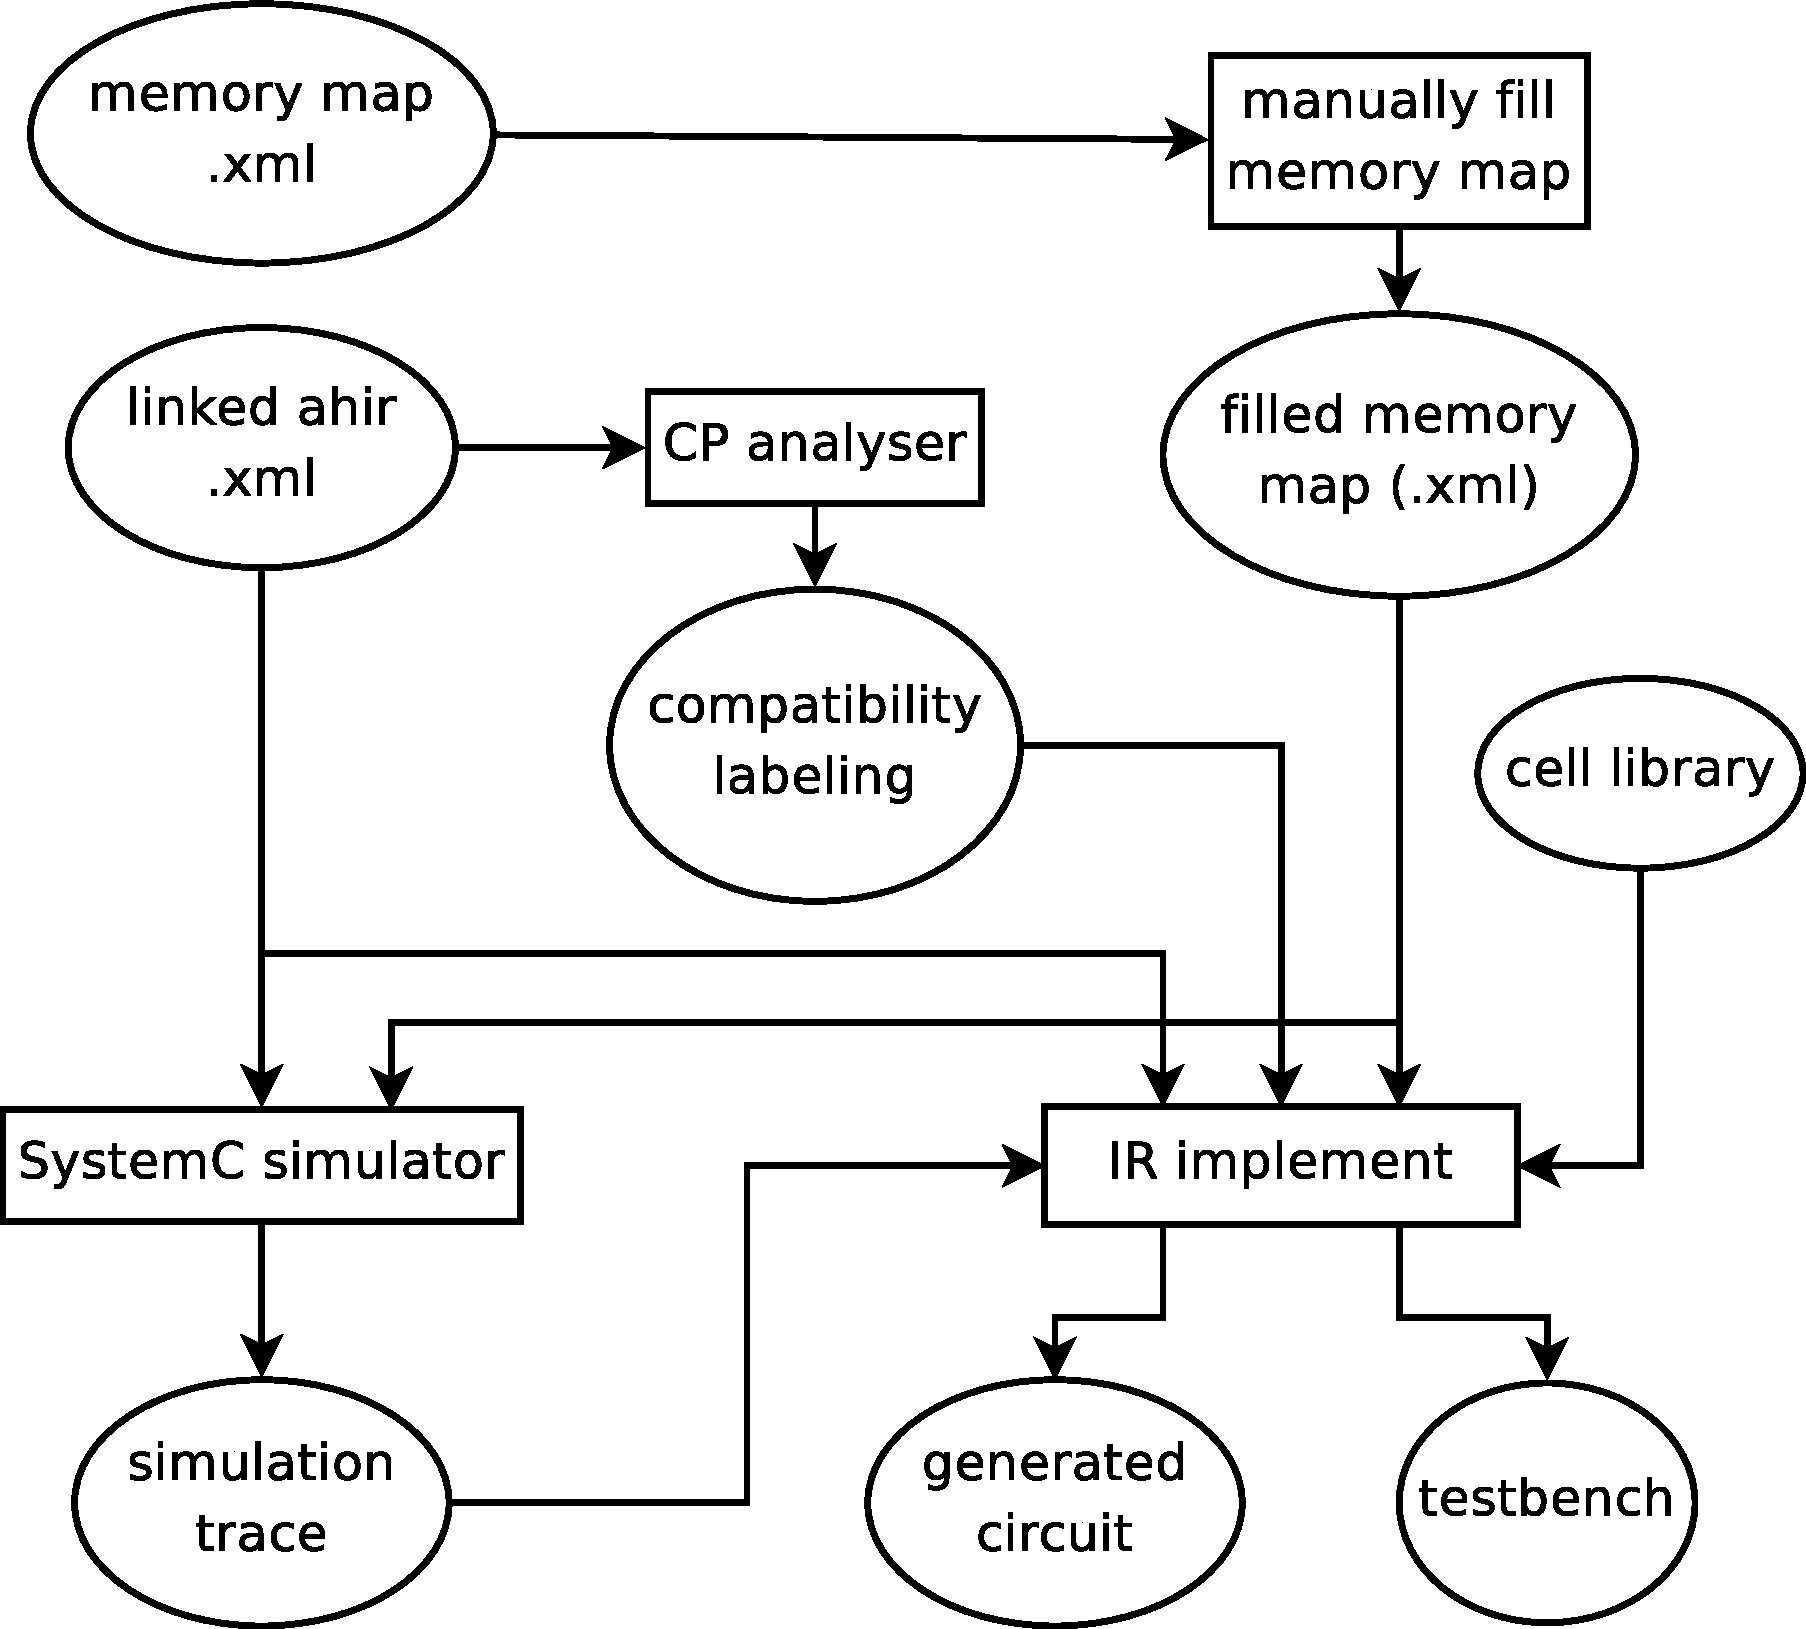
\includegraphics[keepaspectratio,width=4in]{images/simulation-and-synthesis.pdf}
  \caption{Tools for processing an AHIR specification}
  \label{figure:simulation-and-synthesis}
\end{figure}

\section{Expected input}

Currently, the toolchain works with a single C file that contains all
the functions of a program. There are a number of limitations on the C
code accepted.

\subsection{Restrictions imposed by the AHIR platform}

\begin{enumerate}
  \item The program's call-graph should be a DAG. This condition is
        currently not checked, so the result will be undefined if a
        cyclic call-graph is provided as input.
  \item Function pointers are not allowed.
  \item Functions with variable number of arguments are also not
        allowed.
  \item Dynamic memory allocation and other system calls are not
        possible. They may be implemented by an application
        internally, but they are not part of the AHIR platform.
\end{enumerate}

\subsection{Limitations in the current implementation}

\begin{enumerate}
  \item The complete program must be present in a single file.
  \item The complete DAG must contain a function called {\tt start},
        which denotes the root of the call-graph. The function {\tt
        main} should not be used, since it will trigger internal
        modifications by the C front-end, that are incompatible with
        the ahir tools.
  \item Bit selection operators have not been implemented.
\end{enumerate}

\subsection{Fully supported C constructs}

\begin{enumerate}
  \item 32-bit signed and unsigned integers, 32-bit floats and
        pointers (all other sizes are automatically typecast to 32
        bits)
  \item Arithmetic and bit-wise operators
  \item Pointers to data
  \item Structures and arrays
  \item Static memory allocation
  \item Control structures --- \texttt{if-then-else},
        \texttt{while-do}, \texttt{do-while}, \texttt{for},
        \texttt{break} and \texttt{continue}
\end{enumerate}

\subsection{Running example}

The rest of the document assumes an example input file named {\tt
sample.c}. This file contains a C-program with three functions, and a
call-graph as follows:

\[\texttt{start}\rightarrow\texttt{foo}\rightarrow\texttt{bar}\]

\section{Source compiler}

The input C source is parsed by the LLVM front-end, \texttt{llvm-gcc}. 
This produces a bytecode file that contains the input program in
LLVM's native IR. The command is invoked as follows:

\begin{quote}
\tt llvm-gcc sample.c -o sample.bc
\end{quote}

Note that \texttt{llvm-gcc} is part of the LLVM toolkit. It has a
number of command-line options to control its behaviour. The
installation script for the AHIR tools creates an alias in the users
environment that includes all the relevant switches.

\section{AHIR-XML generator}

The LLVM bytecode generated by the front-end is used as the actual
input that is converted into an AHIR specification. The command
\texttt{irgen} is an LLVM-based tool that reads the bytecode, converts
it to AHIR, and generates an XML file describing the AHIR virtual
circuit.

\begin{quote}
  irgen sample.bc
\end{quote}

This produces an XML file, which contains unlinked AHIR-XML
descriptions of the functions \texttt{start}, \texttt{foo} and
\texttt{bar}. It also contains meta-information about the call-graph
that constitutes \texttt{sample.c}

Since \texttt{irgen} is an LLVM tool, it has access to all the
transformations and optimisations that are available as part of the
LLVM framework. These can be specified by command-line arguments to
the \texttt{irgen} command. The entire list of available operations
can be viewed by invoking \texttt{irgen} as follows:

\begin{quote}
\tt  irgen -help
\end{quote}

%When generating the AHIR specification, \texttt{irgen} imposes a few
%structural constraints on the internal representation of the program.
%To enforce these constraints, some LLVM transformations are always
%invoked by \texttt{irgen} just before generating AHIR, but after
%applying the transformations specified on the command line. These
%hardcoded invocations cannot be controlled from the command-line. They
%can only be changed by modifying the utility itself.

\section{AHIR-XML linker}

The unlinked XML specification also includes the call-graph of the
original program. This information is required to provide
predetermined memory locations called \textit{postboxes} used to pass
arguments during function calls. The modules in the unlinked
specification refer to these locations only through names, since their
addresses are not yet known.

The linker assigns numerical addresses to all the postboxes required
for various function calls. In addition, it also creates locations for
global variables as well as statically allocated variables. It is
invoked on the unlinked XML as follows:

\begin{quote}
\tt  irlink sample.xml
\end{quote}

This produces a linked version of the input XML, in a file called
\texttt{sample\_linked.xml}. Additionally, a memory map is created with the
name \texttt{sample\_map.xml}.

The memory map is an XML file that describes known memory locations
ordered by their addresses. The format includes tags used to describe
structured values as well as scalar values. The map itself is divided
in two sections:

\begin{description}
  \item [\texttt{init}:] the initial state of the memory at invocation
        of the circuit
  \item [\texttt{fin}:] the expected state of the memory after
        execution
\end{description}

As a built-in precaution, \texttt{irlink} never over-writes an
existing memory map. When \texttt{irlink} is run, if the file
\texttt{sample\_map.xml} already exists, it instead creates a second
file called \texttt{sample\_new\_map.xml}. This second file is not
protected, and will be over-written by subsequent runs.

\section{SystemC simulator}

The linked AHIR specification can be simulated using SystemC. The
command \texttt{irsim} reads an AHIR description and a memory map, to
generate a set of SystemC modules in-memory. The modules are run until
the control-path of the module for the \texttt{start} function
triggers its \texttt{fin} transition, marking the end of execution.

\begin{quote}
\tt  irsim --ir sample\_linked.xml --map sample\_map.xml
\end{quote}

The simulator uses the \texttt{init} section of the memory map to
initialise the simulated memory, but ignores the contents of the
\texttt{fin} section.

The simulation results in a trace of the memory accesses seen by the
memory subsystem during execution. For each access to the memory
subsystem, the trace records the time of the access along with the
port and the address used.

Note that the simulator does not generate any actual SystemC
description for now. It simply instantiates a SystemC objects that
represent AHIR structures, and directly runs them.

%This has the
%following limitations:

%\begin{enumerate}
%  \item The SystemC ``library'' that implements AHIR is not pluggable.
%  \item Any implementation of arbitrary-width data-types requires
%        the widths to be constant at compile time. For this, the AHIR
%        specification should be translated to a set of SystemC source
%        files, that are then compiled to generate a simulation. As a
%        result, the current implementation can only support a known
%        data-width.
%\end{enumerate}


\section{VHDL generator}

The VHDL generator is a direct mapping of the AHIR specification to an
implementation. The generator creates a VHDL entity for each module in
the specification. These entities use standard names and interfaces to
instantiate and connect building blocks that are assumed to be
available in an independent library.

\begin{quote}
\tt irsyn --ir sample\_linked.xml --map sample\_map.xml
\end{quote}

This will generate the following set of VHDL files:

\begin{itemize}
  \item \texttt{start\_cp.vhdl}, etc --- one control-path for each function
  \item \texttt{start\_dp.vhdl}, etc --- data-path
  \item \texttt{start\_ln.vhdl}, etc --- intra-module link layer
  \item \texttt{omega.vhdl} --- a single inter-module link layer
  \item \texttt{memory.vhdl} --- the memory subsystem
  \item \texttt{system.vhdl} --- built from all of the above
  \item \texttt{testbench.vhdl} --- used to interact with the system
\end{itemize}

The testbench contains an array of values parsed from the
\texttt{init} section of the memory map. These are used to initialise
the memory subsystem. Similarly the testbench also contains values
specified in the \texttt{fin} section, that are used to verify the
contents of the memory at the end of execution.

\end{document}
